% The contents of this file is 
% Copyright (c) 2009-  Charles R. Severance, All Righs Reserved

\chapter{Using databases and Structured Query Language (SQL)}

\section{What is a database?}
\index{database}

A {\bf database} is a file that is organized for storing data.
Most databases are organized like a dictionary in the sense
that they map from keys to values.  The biggest difference
is that the database is on disk (or other permanent storage),
so it persists after the program ends.  Because a database is
stored on permanent storage, it can store far more data than
a dictionary, which is limited to the size of the memory 
in the computer.

\index{database!indexes}
Like a dictionary, database software is designed to keep 
the inserting and accessing of data very fast, even for large
amounts of data.   Database software maintains its performance by 
building {\bf indexes} as data is added to the database
to allow the computer to jump quickly to a particular
entry.

There are many different database systems which are used for a wide
variety of purposes including: Oracle, MySQL, Microsoft SQL Server, 
PostgreSQL, and SQLite.  We focus on SQLite in this book because
it is a very common database and is already built into Python.  
SQLite is designed to be \emph{embedded} into other applications
to provide database support within the application.  For example,
the Firefox browser also uses the SQLite database internally as do 
many other products.

\url{http://sqlite.org/}

SQLite is well suited to some of the data manipulation problems that we 
see in Informatics such as the Twitter spidering application that we 
describe in this chapter.

\section{Database concepts}

When you first look at a database it looks like a 
spreadsheet with multiple sheets.   The primary data structures 
in a database are:
{\bf tables}, {\bf rows}, and {\bf columns}.  

\beforefig
\centerline{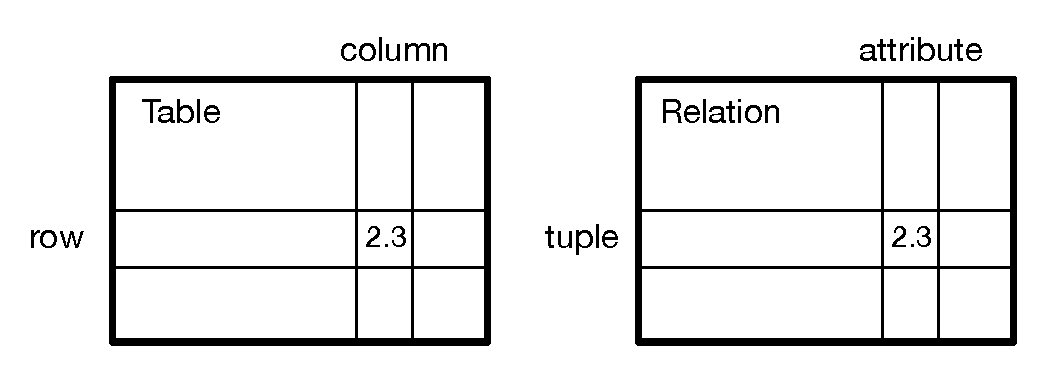
\includegraphics[height=1.50in]{figs2/relational.eps}}
\afterfig

In technical descriptions of relational databases the concepts of 
table, row, and column are more formally referred
to as {\bf relation}, {\bf tuple}, and {\bf attribute}, respectively.
We will use the less formal terms in this chapter.

\section{SQLite manager Firefox add-on}

While this chapter will focus on using Python to work with data 
in SQLite database files, many operations can be done more
conveniently using a Firefox add-on called the {\bf SQLite
Database Manager} which is freely available from:

\url{https://addons.mozilla.org/en-us/firefox/addon/sqlite-manager/}

Using the browser you can easily create tables, insert data, edit data, 
or run simple SQL queries on the data in the database.

In a sense, the database manager is similar to a text editor
when working with text files.   When you want to do one or
very few operations on a text file, you can just open it
in a text editor and make the changes you want.   When you have 
many changes that you need to do to a text file, often you 
will write a simple Python program.  You will find the same 
pattern when working with databases.  You will do simple
operations in the database manager and more complex operations
will be most conveniently done in Python.

\section{Creating a database table}

Databases require more defined structure than Python lists 
or dictionaries\footnote{SQLite actually does allow some 
flexibility in the type of data stored in a column,
but we will keep our data types strict in this chapter
so the concepts apply equally to other database systems 
such as MySQL.}.  

When we create a database {\bf table} we
must tell the database in advance the names of each of the
{\bf columns} in the table and the type of data which we are 
planning to store in each {\bf column}.   When the database software
knows the type of data in each column, it can choose the most 
efficient way to store and look up the data based on the type of
data. 

You can look at the various data types supported by SQLite
at the following url:

\url{http://www.sqlite.org/datatypes.html}

Defining structure for your data up front may seem inconvenient
at the beginning, but the payoff is fast access to your data 
even when the database contains a large amount of data.

The code to create a database file and a table 
named {\tt Tracks} with two columns in the 
database is as follows:

\index{sqlite3 module}
\index{module!sqlite3}
\beforeverb
\begin{verbatim}
import sqlite3

conn = sqlite3.connect('music.sqlite3')
cur = conn.cursor()

cur.execute('DROP TABLE IF EXISTS Tracks ')
cur.execute('CREATE TABLE Tracks (title TEXT, plays INTEGER)')

conn.close()
\end{verbatim}
\afterverb
%
\index{connect function}
\index{function!connect}
\index{cursor function}
\index{function!cursor}
The {\tt connect} operation makes a ``connection'' to the database 
stored in the file {\tt music.sqlite3} in the current directory.   If
the file does not exist, it will be created.  The reason this
is called a ``connection'' is that sometimes the database is stored
on a separate ``database server'' from the server on which we 
are running our application.  In our simple examples 
the database will just be a local file in the same directory
as the Python code we are running.

A {\bf cursor} is like a file handle that we can use to perform
operations on the data stored in the database.  Calling 
{\tt cursor()} is very similar conceptually to calling
{\tt open()} when dealing with text files.

\beforefig
\centerline{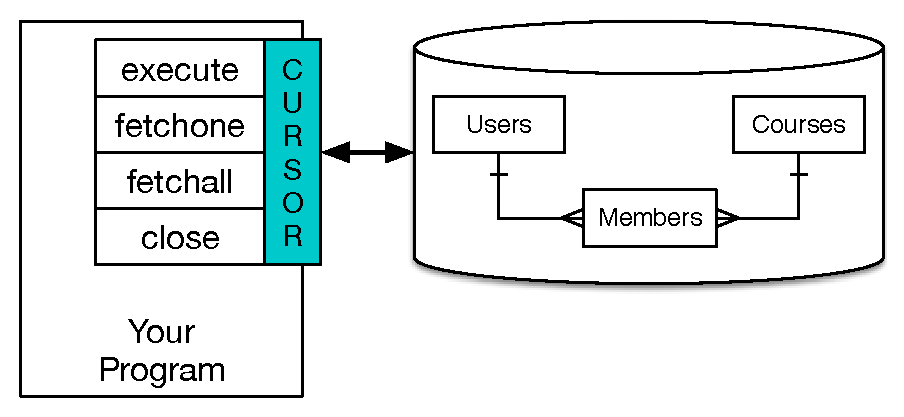
\includegraphics[height=1.50in]{figs2/cursor.eps}}
\afterfig

Once we have the cursor, we can begin to execute 
commands on the contents of the database using the {\tt execute()}
method.

Database commands are expressed in a special language that has 
been standardized across many different database vendors 
to allow us to learn a single database language.   The database
language is called {\bf Structured Query Language} or {\bf SQL}
for short.

\url{http://en.wikipedia.org/wiki/SQL}

In our example, we are executing two SQL commands in our database.
As a convention, we will show the SQL keywords in uppercase 
and the parts of the command that we are adding (such as the
table and column names) will be shown in lowercase.

The first SQL command removes the {\tt Tracks} table from the 
database if it exists.  This pattern is simply to allow us to 
run the same program to create the {\tt Tracks} table over 
and over again without causing an error.  Note that the
{\tt DROP TABLE} command deletes the table and all of its contents
from the database (i.e., there is no ``undo'').

\beforeverb
\begin{verbatim}
cur.execute('DROP TABLE IF EXISTS Tracks ')
\end{verbatim}
\afterverb
%
The second command creates a table named
{\tt Tracks} with a text column named {\tt title}
and an integer column named {\tt plays}.

\beforeverb
\begin{verbatim}
cur.execute('CREATE TABLE Tracks (title TEXT, plays INTEGER)')
\end{verbatim}
\afterverb
%
Now that we have created a table named {\tt Tracks}, we can put some data
into that table using the SQL {\tt INSERT} operation.   Again, we begin
by making a connection to the database and obtaining the {\tt cursor}.
We can then execute SQL commands using the cursor.

The SQL {\tt INSERT} command indicates which table we are using 
and then defines a new row by listing the fields we want to 
include {\tt (title, plays)} followed by the {\tt VALUES} we want
placed in the new row.  We specify the values as question marks
{\tt (?, ?)} to indicate that the actual values are passed in as a
tuple {\tt ( 'My Way', 15 ) } as the second parameter to the
{\tt execute()} call.

\beforeverb
\begin{verbatim}
import sqlite3

conn = sqlite3.connect('music.sqlite3')
cur = conn.cursor()

cur.execute('INSERT INTO Tracks (title, plays) VALUES ( ?, ? )', 
    ( 'Thunderstruck', 20 ) )
cur.execute('INSERT INTO Tracks (title, plays) VALUES ( ?, ? )', 
    ( 'My Way', 15 ) )
conn.commit()

print 'Tracks:'
cur.execute('SELECT title, plays FROM Tracks')
for row in cur :
   print row

cur.execute('DELETE FROM Tracks WHERE plays < 100')
conn.commit()

cur.close()
\end{verbatim}
\afterverb
%
First we {\tt INSERT} two rows into our table and use {\tt commit()} 
to force the data to be written to the database file.

\beforefig
\centerline{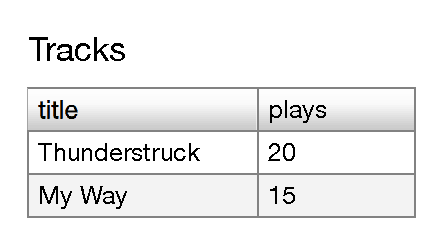
\includegraphics[height=1.00in]{figs2/tracks.eps}}
\afterfig

Then we use the {\tt SELECT} command
to retrieve the rows we just inserted from the table.  
On the 
{\tt SELECT} command, we indicate which columns we would like {\tt (title, plays)}
and indicate which table we want to retrieve the data from.  After we 
execute the {\tt SELECT} statement, the cursor is something we can loop through
in a {\tt for} statement.   For efficiency,
the cursor does not read all of the data from the
database when we execute the {\tt SELECT} statement.  
Instead, the data is read on demand
as we loop through the rows in the {\tt for} statement.

The output of the program is as follows:

\beforeverb
\begin{verbatim}
Tracks:
(u'Thunderstruck', 20)
(u'My Way', 15)
\end{verbatim}
\afterverb
%
\index{Unicode}
Our {\tt for} loop finds two rows, and each row is a Python tuple with the
first value as the {\tt title} and the second value as the number of {\tt plays}.
Do not be concerned that the title strings are shown starting with 
{\tt u'}.  This is an indication that the strings are {\bf Unicode} strings
that are capable of storing non-Latin character sets.

At the very end of the program, we execute an SQL command to {\tt DELETE} 
the rows we have just created so we can run the program over and over.
The {\tt DELETE} command shows the use of a {\tt WHERE} clause that
allows us to express a selection criterion so that we can ask the database
to apply the command to only the rows that match the criterion.  In this example
the criterion happens to apply to all the rows so we empty the table
out so we can run the program repeatedly.  After the {\tt DELETE} is performed,
we also call {\tt commit()} to force the data to be removed from the database.

\section{Structured Query Language summary}

So far, we have been using the Structured Query Language in our Python
examples and have covered many of the basics of the SQL commands.
In this section, we look at the SQL language in particular
and give an overview of SQL syntax.

Since there are so many different database vendors, the Structured Query
Language (SQL) was standardized so we could communicate in a portable
manner to database systems from multiple vendors.

A relational database is made up of tables, rows, and columns.  The columns
generally have a type such as text, numeric, or date data.  When we create
a table, we indicate the names and types of the columns:

\beforeverb
\begin{verbatim}
CREATE TABLE Tracks (title TEXT, plays INTEGER)
\end{verbatim}
\afterverb
%
To insert a row into a table, we use the SQL {\tt INSERT} command:

\beforeverb
\begin{verbatim}
INSERT INTO Tracks (title, plays) VALUES ('My Way', 15)
\end{verbatim}
\afterverb
%
The {\tt INSERT} statement specifies the table name, then a list of
the fields/columns that you would like to set in the new row, and then 
the keyword {\tt VALUES} and a list of corresponding values 
for each of the fields.

The SQL {\tt SELECT} command is used to retrieve rows and columns from a database.
The {\tt SELECT} statement lets you specify which columns you would
like to retrieve as well as a {\tt WHERE} clause to select which 
rows you would like to see.  It also allows an optional 
{\tt ORDER BY} clause to control the sorting of the returned rows.

\beforeverb
\begin{verbatim}
SELECT * FROM Tracks WHERE title = 'My Way'
\end{verbatim}
\afterverb
%
Using \verb"*" indicates that you want the database to return all of 
the columns for each row that matches the {\tt WHERE} clause.  

Note, unlike in Python, in a SQL {\tt WHERE} clause 
we use a single equal sign 
to indicate a test for equality rather than a double equal sign.
Other logical operations allowed in a {\tt WHERE} clause include 
\verb"<",
\verb">",
\verb"<=",
\verb">=",
\verb"!=",
as well as {\tt AND} and {\tt OR} and parentheses
to build your logical expressions.

You can request that the returned rows be sorted by one of 
the fields as follows:

\beforeverb
\begin{verbatim}
SELECT title,plays FROM Tracks ORDER BY title
\end{verbatim}
\afterverb
%
To remove a row, you need a {\tt WHERE} clause on an SQL {\tt DELETE}
statement.  The {\tt WHERE} clause determines which rows are to be deleted:

\beforeverb
\begin{verbatim}
DELETE FROM Tracks WHERE title = 'My Way'
\end{verbatim}
\afterverb
%
It is possible to {\tt UPDATE} a column or columns within one or more rows
in a table using the SQL {\tt UPDATE} statement as follows:

\beforeverb
\begin{verbatim}
UPDATE Tracks SET plays = 16 WHERE title = 'My Way'
\end{verbatim}
\afterverb
%
The {\tt UPDATE} statement specifies a table and 
then a list of fields and values to change after the {\tt SET} 
keyword and then an optional {\tt WHERE} clause to select
the rows that are to be updated.  A single {\tt UPDATE} statement
will change all of the rows that match the {\tt WHERE} clause.  If 
a {\tt WHERE} clause is not specified, it performs the {\tt UPDATE}
on all of the rows in the table.

These four basic SQL commands (INSERT, SELECT, UPDATE, and DELETE) allow 
the four basic operations needed to create and maintain data.


\section{Spidering Twitter using a database}

In this section, we will create a simple spidering program that will 
go through Twitter accounts and build a database of them.
\emph{Note: Be very careful when running this program.  You do not
want to pull too much data or run the program for too long and
end up having your Twitter access shut off.}

One of the problems of any kind of spidering program is that it 
needs to be able to be stopped and restarted many times and 
you do not want to lose the data that you have retrieved so far.
You don't want to always restart your data retrieval at the
very beginning so we want to store data as we retrieve it so our
program can start back up and pick up where it left off.

We will start by retrieving one person's Twitter friends and their
statuses, looping through the list of friends, and adding each 
of the friends to a database to be retrieved in the future.  After
we process one person's Twitter friends, we check in our database
and retrieve one of the friends of the friend.  We do this over and
over, picking an ``unvisited'' person, retrieving their friend list,
and adding friends we have not seen to our list for a future visit.

We also track how many times we have seen a particular friend in the
database to get some sense of their ``popularity''.

By storing our list of known accounts and whether 
we have retrieved the account or not, 
and how popular the account is in a database on the disk
of the computer, we can stop and
restart our program as many times as we like.

% TODO: Add a reference to the right spot
This program is a bit complex. It is based on the code 
from the exercise earlier in the book that uses
the Twitter API.

Here is the source code for our Twitter spidering application:

\beforeverb
\begin{verbatim}
import urllib
import twurl
import json
import sqlite3

TWITTER_URL = 'https://api.twitter.com/1.1/friends/list.json'

conn = sqlite3.connect('spider.sqlite3')
cur = conn.cursor()

cur.execute('''
CREATE TABLE IF NOT EXISTS Twitter 
(name TEXT, retrieved INTEGER, friends INTEGER)''')

while True:
    acct = raw_input('Enter a Twitter account, or quit: ')
    if ( acct == 'quit' ) : break
    if ( len(acct) < 1 ) :
        cur.execute('SELECT name FROM Twitter WHERE retrieved = 0 LIMIT 1')
        try:
            acct = cur.fetchone()[0]
        except:
            print 'No unretrieved Twitter accounts found'
            continue

    url = twurl.augment(TWITTER_URL, 
               {'screen_name': acct, 'count': '20'} )
    print 'Retrieving', url
    connection = urllib.urlopen(url)
    data = connection.read()
    headers = connection.info().dict
    # print 'Remaining', headers['x-rate-limit-remaining']
    js = json.loads(data)
    # print json.dumps(js, indent=4)

    cur.execute('UPDATE Twitter SET retrieved=1 WHERE name = ?', (acct, ) )

    countnew = 0
    countold = 0
    for u in js['users'] :
        friend = u['screen_name']
        print friend
        cur.execute('SELECT friends FROM Twitter WHERE name = ? LIMIT 1', 
            (friend, ) )
        try:
            count = cur.fetchone()[0]
            cur.execute('UPDATE Twitter SET friends = ? WHERE name = ?', 
                (count+1, friend) )
            countold = countold + 1
        except:
            cur.execute('''INSERT INTO Twitter (name, retrieved, friends) 
                VALUES ( ?, 0, 1 )''', ( friend, ) )
            countnew = countnew + 1
    print 'New accounts=',countnew,' revisited=',countold
    conn.commit()

cur.close()
\end{verbatim}
\afterverb
%
Our database is stored in the file {\tt spider.sqlite3} and it has one 
table named {\tt Twitter}.  Each row in the {\tt Twitter} table
has a column for the account name, whether we have retrieved the friends
of this account, and how many times this account has been ``friended''.

In the main loop of the program, we prompt the user for a Twitter
account name or ``quit'' to exit the program.  
If the user enters a Twitter account, we retrieve the 
list of friends and statuses
for that user and add each friend to the database if 
not already in the database.  If the friend is already in the list, 
we add 1 to the {\tt friends} field in the row in the database.

If the user presses enter, we look in the database for the next 
Twitter account that we have not yet retrieved, retrieve the
friends and statuses for that account, add them to the database 
or update them, and increase their {\tt friends} count.

Once we retrieve the list of friends and statuses, we loop 
through all of the {\tt user} items in the returned JSON
and retrieve the \verb"screen_name" for each user.  Then we use
the {\tt SELECT} statement to see if we already have stored this
particular \verb"screen_name" in the database and retrieve the
friend count ({\tt friends}) if the record exists.

\beforeverb
\begin{verbatim}
    countnew = 0
    countold = 0
    for u in js['users'] :
        friend = u['screen_name']
        print friend
        cur.execute('SELECT friends FROM Twitter WHERE name = ? LIMIT 1', 
            (friend, ) )
        try:
            count = cur.fetchone()[0]
            cur.execute('UPDATE Twitter SET friends = ? WHERE name = ?', 
                (count+1, friend) )
            countold = countold + 1
        except:
            cur.execute('''INSERT INTO Twitter (name, retrieved, friends) 
                VALUES ( ?, 0, 1 )''', ( friend, ) )
            countnew = countnew + 1
    print 'New accounts=',countnew,' revisited=',countold
    conn.commit()
\end{verbatim}
\afterverb
%
Once the cursor executes the {\tt SELECT} statement, 
we must retrieve the rows.  We could do this with a {\tt for} 
statement, but since we are only retrieving
one row ({\tt LIMIT 1}), we can use the {\tt fetchone()} method to fetch the
first (and only) row that is the result of the {\tt SELECT} operation.  
Since {\tt fetchone()} returns the row as a {\bf tuple} (even though there is only
one field), we take the first value from the tuple using {\tt [0]} to get the 
current friend count into the variable {\tt count}.  

If this retrieval is successful, we use the SQL {\tt UPDATE} statement with a 
{\tt WHERE} clause to add 1 to the {\tt friends} column for the row that 
matches the friend's account.  Notice that there are two placeholders (i.e.,
question marks) in the SQL, and the second parameter to the {\tt execute()} is
a two-element tuple that holds the values to be substituted into the SQL
in place of the question marks.

If the code in the {\tt try} block fails, it is probably because no record
matched the {\tt WHERE name = ?} clause on the SELECT statement.  So in the
{\tt except} block, we use the SQL {\tt INSERT} statement to add the friend's
\verb"screen_name" to the table with an indication that we have not yet 
retrieved the \verb"screen_name" and set the friend count to zero.

So the first time the program runs and we enter a Twitter account, the program
runs as follows:

\beforeverb
\begin{verbatim}
Enter a Twitter account, or quit: drchuck
Retrieving http://api.twitter.com/1.1/friends ...
New accounts= 20  revisited= 0
Enter a Twitter account, or quit: quit
\end{verbatim}
\afterverb
%
Since this is the first time we have run the program, the database
is empty and we create the database in the file {\tt spider.sqlite3} and
add a table named {\tt Twitter} to the database.  Then we retrieve
some friends and add them all to the database since the database is
empty.

At this point, we might want to write a simple database dumper
to take a look at what is in our {\tt spider.sqlite3} file:

\beforeverb
\begin{verbatim}
import sqlite3

conn = sqlite3.connect('spider.sqlite3')
cur = conn.cursor()
cur.execute('SELECT * FROM Twitter')
count = 0
for row in cur :
   print row
   count = count + 1
print count, 'rows.'
cur.close()
\end{verbatim}
\afterverb
%
This program simply opens the database and selects all of the 
columns of all of the rows in the table {\tt Twitter}, then 
loops through the rows and prints out each row.

If we run this program after the first execution of our Twitter
spider above, its output will be as follows:

\beforeverb
\begin{verbatim}
(u'opencontent', 0, 1)
(u'lhawthorn', 0, 1)
(u'steve_coppin', 0, 1)
(u'davidkocher', 0, 1)
(u'hrheingold', 0, 1)
...
20 rows.
\end{verbatim}
\afterverb
%
We see one row for each \verb"screen_name", that we 
have not retrieved the data for that \verb"screen_name", and 
everyone in the database has one friend.

Now our database reflects the retrieval of the friends of 
our first Twitter account ({\bf drchuck}).  We can run the program
again and tell it to retrieve the friends of the next 
``unprocessed'' account by simply pressing enter instead of
a Twitter account as follows:

\beforeverb
\begin{verbatim}
Enter a Twitter account, or quit: 
Retrieving http://api.twitter.com/1.1/friends ...
New accounts= 18  revisited= 2
Enter a Twitter account, or quit: 
Retrieving http://api.twitter.com/1.1/friends ...
New accounts= 17  revisited= 3
Enter a Twitter account, or quit: quit
\end{verbatim}
\afterverb
%
Since we pressed enter (i.e., we did not specify a Twitter account),
the following code is executed:

\beforeverb
\begin{verbatim}
    if ( len(acct) < 1 ) :
        cur.execute('SELECT name FROM Twitter WHERE retrieved = 0 LIMIT 1')
        try:
            acct = cur.fetchone()[0]
        except:
            print 'No unretrieved twitter accounts found'
            continue
\end{verbatim}
\afterverb
%
We use the SQL {\tt SELECT} statement to retrieve the name of the first 
({\tt LIMIT 1}) user who still has their ``have we retrieved this user''
value set to zero.  We also use the {\tt fetchone()[0]} pattern within 
a try/except block to either extract a \verb"screen_name" from the retrieved
data or put out an error message and loop back up.

If we successfully retrieved an unprocessed \verb"screen_name", we retrieve
their data as follows:

\beforeverb
\begin{verbatim}
    url = twurl.augment(TWITTER_URL, {'screen_name': acct, 'count': '20'} )
    print 'Retrieving', url
    connection = urllib.urlopen(url)
    data = connection.read()
    js = json.loads(data)

    cur.execute('UPDATE Twitter SET retrieved=1 WHERE name = ?', (acct, ) )
\end{verbatim}
\afterverb
%
Once we retrieve the data successfully, we use the {\tt UPDATE} statement 
to set the {\tt retrieved} column to 1 to indicate that we have completed 
the retrieval of the friends of this account.  This keeps us from retrieving
the same data over and over and keeps us progressing forward through the network
of Twitter friends.

If we run the friend program and press enter twice to retrieve the next 
unvisited friend's friends,
then run the dumping program, it will give us the following output:

\beforeverb
\begin{verbatim}
(u'opencontent', 1, 1)
(u'lhawthorn', 1, 1)
(u'steve_coppin', 0, 1)
(u'davidkocher', 0, 1)
(u'hrheingold', 0, 1)
...
(u'cnxorg', 0, 2)
(u'knoop', 0, 1)
(u'kthanos', 0, 2)
(u'LectureTools', 0, 1)
...
55 rows.
\end{verbatim}
\afterverb
%
We can see that we have properly recorded that we have visited 
{\tt lhawthorn} and {\tt opencontent}.  Also the accounts 
{\tt cnxorg} and {\tt kthanos} already have two followers.
Since we now have retrieved the friends of three people
({\tt drchuck}, {\tt opencontent}, and {\tt lhawthorn}) our table has 55 rows 
of friends to retrieve.

Each time we run the program and press enter it will pick the next 
unvisited account (e.g., the next account will be \verb"steve_coppin"),
retrieve their friends, mark them as retrieved, and for each of the 
friends of \verb"steve_coppin" either add them to the end of the 
database or update their friend count if they are already in the
database.

Since the program's data is all stored on disk in a database, 
the spidering activity can be suspended and resumed as many times as you 
like with no loss of data.

\section{Basic data modeling}

The real power of a relational database is when we create multiple tables
and make links between those tables.   The act of deciding how to break
up your application data into multiple tables and establishing the
relationships between the tables is called {\bf data modeling}.  The
design document that shows the tables and their relationships 
is called a {\bf data model}.

Data modeling is a relatively sophisticated skill and we will only introduce
the most basic concepts of relational data modeling in this section.  For more
detail on data modeling you can start with:

\url{http://en.wikipedia.org/wiki/Relational_model}

Let's say for our Twitter spider application, instead of just 
counting a person's friends, we wanted to keep a list of 
all of the incoming relationships so we could find a list of 
everyone who is following a particular account.

Since everyone will potentially have many accounts that follow
them, we cannot simply add a single column to our {\tt Twitter} table. 
So we create a new table that keeps track of pairs of friends.
The following is a simple way of making such a table:

\beforeverb
\begin{verbatim}
CREATE TABLE Pals (from_friend TEXT, to_friend TEXT)
\end{verbatim}
\afterverb
%
Each time we encounter a person who {\tt drchuck} is following, we
would insert a row of the form:

\beforeverb
\begin{verbatim}
INSERT INTO Pals (from_friend,to_friend) VALUES ('drchuck', 'lhawthorn')
\end{verbatim}
\afterverb
%
As we are processing the 20 friends from the {\tt drchuck}
Twitter feed, we will insert 20 records with ``drchuck''
as the first parameter so we will end up duplicating the 
string many times in the database.

This duplication of string data violates one of the best practices 
for {\bf database normalization} which basically states that
we should never put the same string data in the database more than once.  
If we need the data more than once, we create a 
numeric {\bf key} for the data and reference the actual data 
using this key.

In practical terms, a string takes up a lot more 
space than an integer on the disk
and in the memory of our computer, and takes more processor time
to compare and sort.  If we only have a few hundred entries, 
the storage and processor time hardly matters.  But if we have 
a million people in our database and a possibility of 100 million
friend links, it is important to be able to scan data as quickly
as possible.

We will store our Twitter accounts in a table named {\tt People}
instead of the {\tt Twitter} table used in the previous example.
The {\tt People} table has an additional column 
to store the numeric key associated with the 
row for this Twitter user.   
SQLite has a feature that automatically adds the key value
for any row we insert into a table using a special type of 
data column ({\tt INTEGER PRIMARY KEY}).

We can create the {\tt People} table with this additional 
{\tt id} column as follows:

\beforeverb
\begin{verbatim}
CREATE TABLE People 
    (id INTEGER PRIMARY KEY, name TEXT UNIQUE, retrieved INTEGER)
\end{verbatim}
\afterverb
%
Notice that we are no longer maintaining a friend count in each row
of the {\tt People} table.
When we select {\tt INTEGER PRIMARY KEY} as the type of our {\tt id} column,
we are indicating that we would like SQLite to manage this column and 
assign a unique numeric key to each row we insert automatically.
We also add the keyword {\tt UNIQUE} to indicate that we will not 
allow SQLite to insert two rows with the same value for {\tt name}.

Now instead of creating the table {\tt Pals} above, we create
a table called {\tt Follows} with two integer columns
\verb"from_id" and \verb"to_id" and a constraint on the table that
the \emph{combination} of \verb"from_id" and \verb"to_id" must be unique 
in this table (i.e., we cannot insert duplicate rows) in our database.

\beforeverb
\begin{verbatim}
CREATE TABLE Follows 
    (from_id INTEGER, to_id INTEGER, UNIQUE(from_id, to_id) )
\end{verbatim}
\afterverb
%
When we add {\tt UNIQUE} clauses to our tables, we are communicating a set
of rules that we are asking the database to enforce when we attempt to insert
records.   We are creating these rules as a convenience in our programs, as we
will see in a moment.  The rules both keep us from making mistakes and make
it simpler to write some of our code.

In essence, in creating this {\tt Follows} table, we are modelling a 
``relationship'' where one person ``follows'' someone else
and representing it with a pair of numbers indicating that (a) the people are
connected and (b) the direction of the relationship.

\beforefig
\centerline{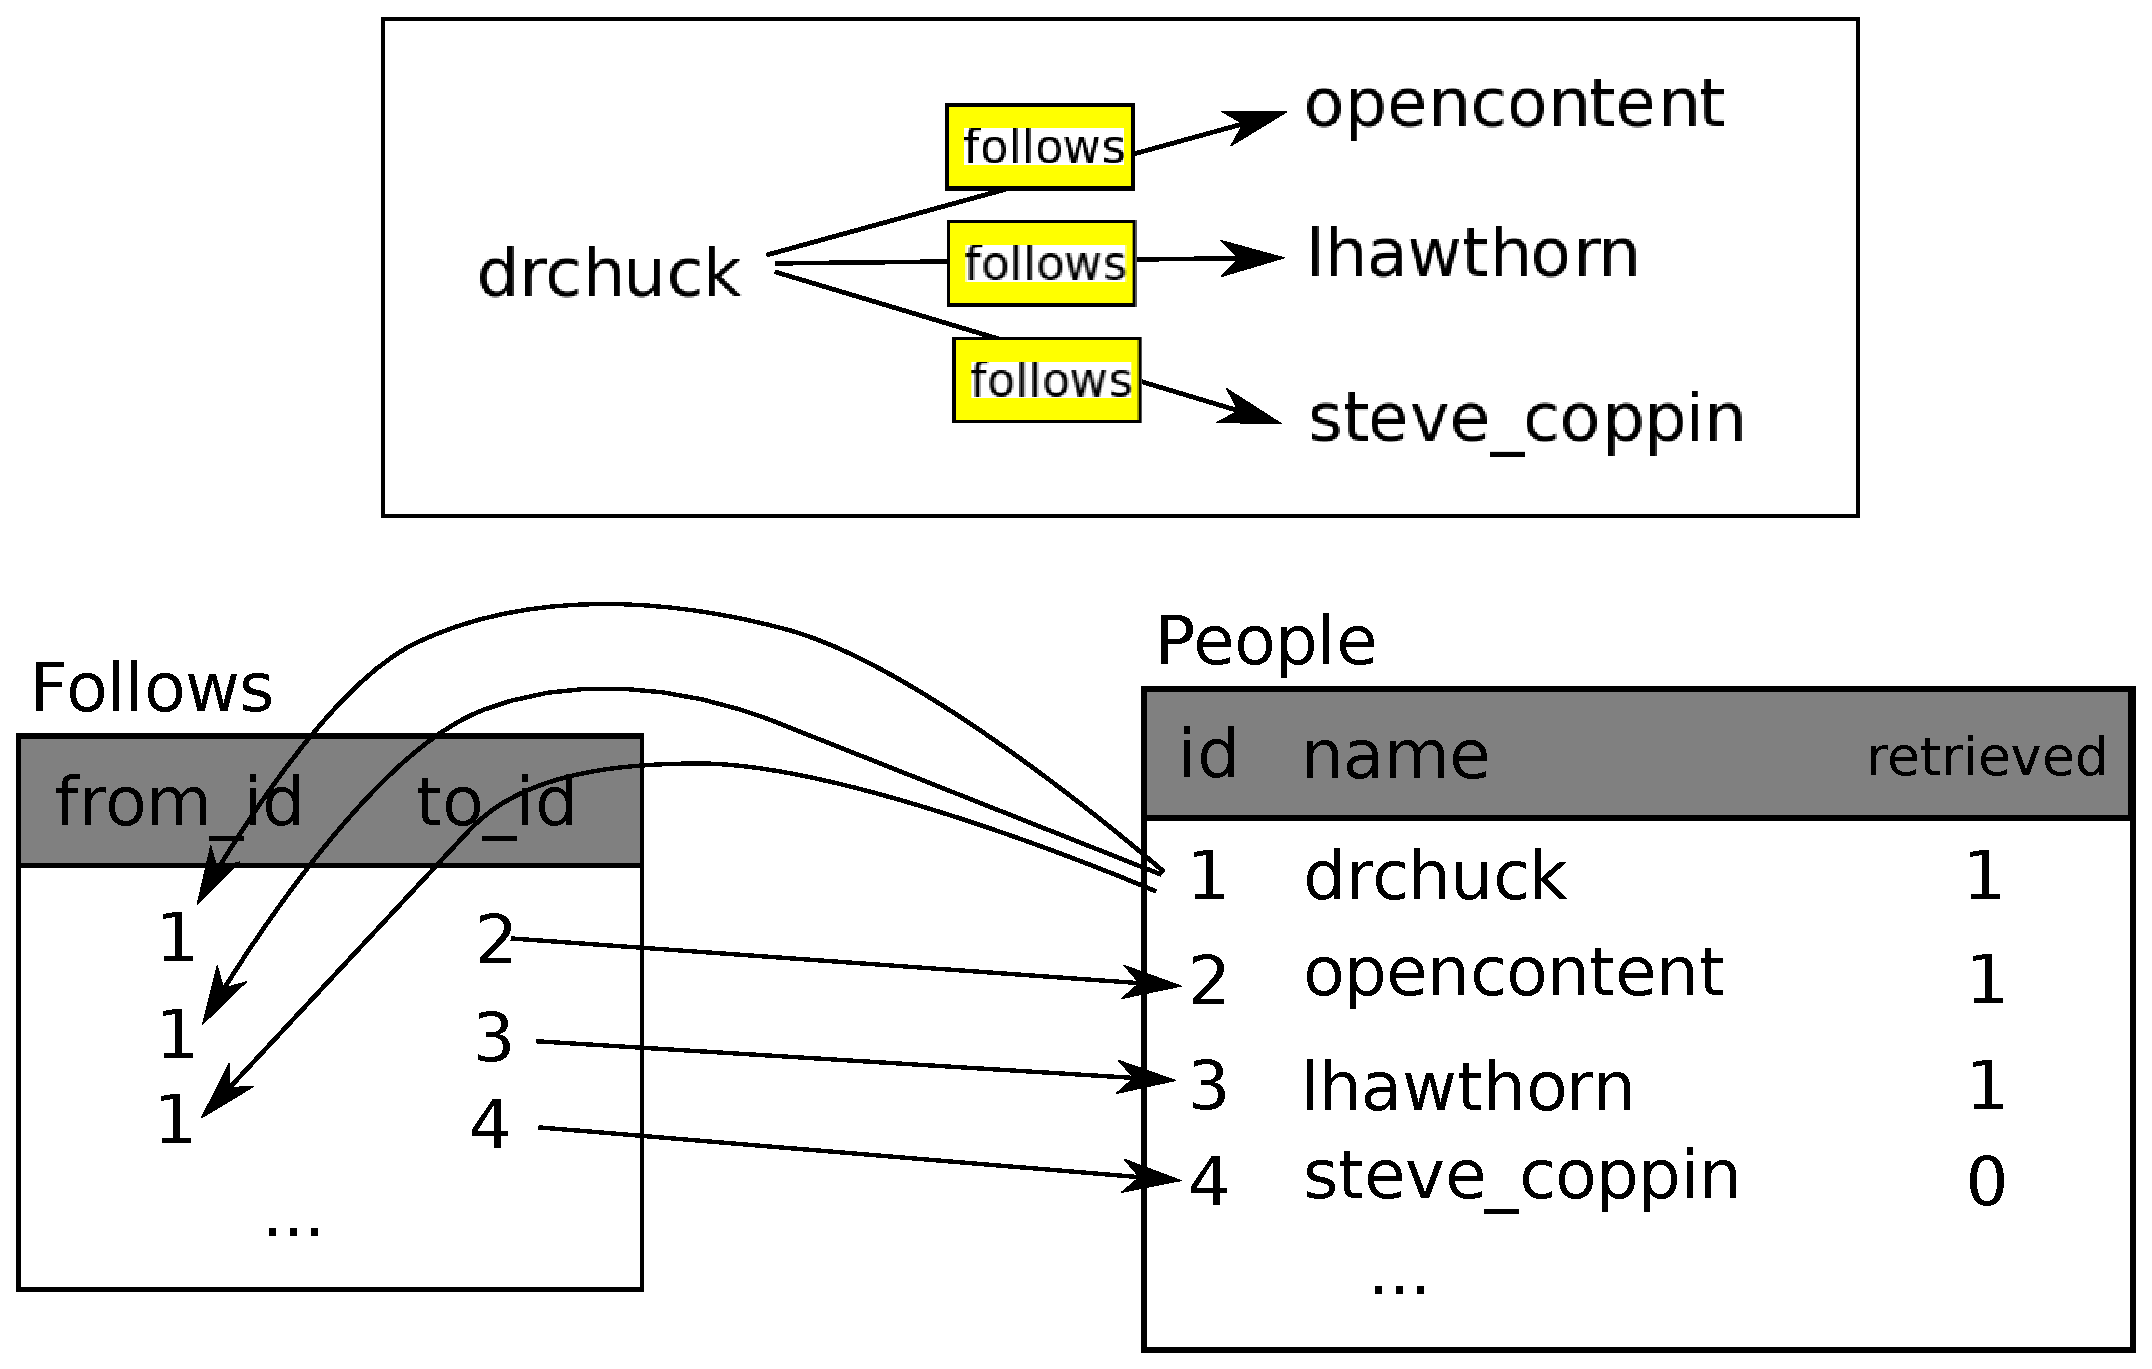
\includegraphics[height=2.50in]{figs2/twitter.eps}}
\afterfig


\section{Programming with multiple tables}

We will now redo the Twitter spider program using two tables, the primary
keys, and the key references as described above.  Here is the code for 
the new version of the program:

\beforeverb
\begin{verbatim}
import urllib
import twurl
import json
import sqlite3

TWITTER_URL = 'https://api.twitter.com/1.1/friends/list.json'

conn = sqlite3.connect('friends.sqlitesqlite3')
cur = conn.cursor()

cur.execute('''CREATE TABLE IF NOT EXISTS People 
    (id INTEGER PRIMARY KEY, name TEXT UNIQUE, retrieved INTEGER)''')
cur.execute('''CREATE TABLE IF NOT EXISTS Follows 
    (from_id INTEGER, to_id INTEGER, UNIQUE(from_id, to_id))''')

while True:
    acct = raw_input('Enter a Twitter account, or quit: ')
    if ( acct == 'quit' ) : break
    if ( len(acct) < 1 ) :
        cur.execute('''SELECT id, name FROM People 
            WHERE retrieved = 0 LIMIT 1''')
        try:
            (id, acct) = cur.fetchone()
        except:
            print 'No unretrieved Twitter accounts found'
            continue
    else:
        cur.execute('SELECT id FROM People WHERE name = ? LIMIT 1', 
            (acct, ) )
        try:
            id = cur.fetchone()[0]
        except:
            cur.execute('''INSERT OR IGNORE INTO People (name, retrieved) 
                VALUES ( ?, 0)''', ( acct, ) )
            conn.commit()
            if cur.rowcount != 1 : 
                print 'Error inserting account:',acct
                continue
            id = cur.lastrowid

    url = twurl.augment(TWITTER_URL, 
       {'screen_name': acct, 'count': '20'} )
    print 'Retrieving account', acct
    connection = urllib.urlopen(url)
    data = connection.read()
    headers = connection.info().dict
    print 'Remaining', headers['x-rate-limit-remaining']

    js = json.loads(data)
    # print json.dumps(js, indent=4)

    cur.execute('UPDATE People SET retrieved=1 WHERE name = ?', (acct, ) )

    countnew = 0
    countold = 0
    for u in js['users'] :
        friend = u['screen_name']
        print friend
        cur.execute('SELECT id FROM People WHERE name = ? LIMIT 1', 
            (friend, ) )
        try:
            friend_id = cur.fetchone()[0]
            countold = countold + 1
        except:
            cur.execute('''INSERT OR IGNORE INTO People (name, retrieved) 
                VALUES ( ?, 0)''', ( friend, ) )
            conn.commit()
            if cur.rowcount != 1 :
                print 'Error inserting account:',friend
                continue
            friend_id = cur.lastrowid
            countnew = countnew + 1
        cur.execute('''INSERT OR IGNORE INTO Follows (from_id, to_id) 
            VALUES (?, ?)''', (id, friend_id) )
    print 'New accounts=',countnew,' revisited=',countold
    conn.commit()

cur.close()
\end{verbatim}
\afterverb
%
This program is starting to get a bit complicated, but it illustrates
the patterns that we need to use when we are
using integer keys to link tables. The basic patterns are:

\begin{enumerate}

\item Create tables with primary keys and constraints.

\item When we have a logical key for a person (i.e., account
name) and we need the {\tt id} value for the person,
depending on whether or not the person is already
in the {\tt People} table we either need to: 
(1) look up the person in the {\tt People} table and 
retrieve the {\tt id} value for the person 
or (2) add the person to the {\tt People} table and get the 
{\tt id} value for the newly added row.

\item Insert the row that captures the ``follows'' relationship.

\end{enumerate}

We will cover each of these in turn.

\subsection{Constraints in database tables}

As we design our table structures, we can tell the database system 
that we would like it to enforce a few rules on us.   These rules
help us from making mistakes and introducing incorrect data into 
out tables.   When we create our tables:

\beforeverb
\begin{verbatim}
cur.execute('''CREATE TABLE IF NOT EXISTS People 
    (id INTEGER PRIMARY KEY, name TEXT UNIQUE, retrieved INTEGER)''')
cur.execute('''CREATE TABLE IF NOT EXISTS Follows 
    (from_id INTEGER, to_id INTEGER, UNIQUE(from_id, to_id))''')
\end{verbatim}
\afterverb
%
We indicate that the {\tt name} column in the {\tt People} table must be
{\tt UNIQUE}.   We also indicate that the combination of the two numbers
in each row of the {\tt Follows} table must be unique.  These constraints
keep us from making mistakes such as adding the same relationship more than
once.

We can take advantage of these constraints in the following code:

\beforeverb
\begin{verbatim}
cur.execute('''INSERT OR IGNORE INTO People (name, retrieved) 
    VALUES ( ?, 0)''', ( friend, ) )
\end{verbatim}
\afterverb
%
We add the {\tt OR IGNORE} clause to our {\tt INSERT} statement to indicate
that if this particular {\tt INSERT} would cause a violation of the
``{\tt name} must be unique'' rule, the database system is allowed to ignore the 
{\tt INSERT}.  We are using the database constraint as a safety net
to make sure we don't inadvertently do something incorrect.

Similarly, the following code ensures that we don't add the 
exact same {\tt Follows} relationship twice.

\beforeverb
\begin{verbatim}
cur.execute('''INSERT OR IGNORE INTO Follows 
    (from_id, to_id) VALUES (?, ?)''', (id, friend_id) )
\end{verbatim}
\afterverb
%
Again, we simply tell the database to ignore our attempted 
{\tt INSERT} if it would violate the uniqueness constraint
that we specified for the {\tt Follows} rows.

\subsection{Retrieve and/or insert a record}

When we prompt the user for a Twitter account, if the account 
exists, we must look up its {\tt id} value.  If the account
does not yet exist in the {\tt People} table, we must insert 
the record and get the {\tt id} value from the inserted
row.

This is a very common pattern and is done twice in the program above.
This code shows how we look up the {\tt id} for a 
friend's account when we have extracted a \verb"screen_name"
from a {\tt user} node in the retrieved Twitter JSON.

Since over time it will be increasingly likely that the account
will already be in the database, we first check to see if the
{\tt People} record exists using a {\tt SELECT} statement.

If all goes well\footnote{In general, when a sentence starts 
with ``if all goes well'' you will find that the code needs
to use try/except.} inside the {\tt try} section, we retrieve the
record using {\tt fetchone()} and then retrieve the
first (and only) element of the returned tuple and store it in 
\verb"friend_id".

If the {\tt SELECT} fails, the {\tt fetchone()[0]} code will fail
and control will transfer into the {\tt except} section.

\beforeverb
\begin{verbatim}
        friend = u['screen_name']
        cur.execute('SELECT id FROM People WHERE name = ? LIMIT 1',
            (friend, ) )
        try:
            friend_id = cur.fetchone()[0]
            countold = countold + 1
        except:
            cur.execute('''INSERT OR IGNORE INTO People (name, retrieved) 
                VALUES ( ?, 0)''', ( friend, ) )
            conn.commit()
            if cur.rowcount != 1 :
                print 'Error inserting account:',friend
                continue
            friend_id = cur.lastrowid
            countnew = countnew + 1
\end{verbatim}
\afterverb
%
If we end up in the {\tt except} code, it simply means that the row
was not found, so we must insert the row.  We use {\tt INSERT OR 
IGNORE} just to avoid errors and then call {\tt commit()} to 
force the database to really be updated.  After the write is done, we can 
check the {\tt cur.rowcount} to see how many rows were affected.  Since
we are attempting to insert a single row, if the number of 
affected rows is something other than 1, it is an error.  

If the {\tt INSERT} is successful, we can look at {\tt cur.lastrowid} 
to find out what value the database assigned to the {\tt id} column in 
our newly created row.

\subsection{Storing the friend relationship}

Once we know the key value for both the Twitter user
and the friend in the JSON, it is a simple matter to insert
the two numbers into the {\tt Follows} table
with the following code:

\beforeverb
\begin{verbatim}
cur.execute('INSERT OR IGNORE INTO Follows (from_id, to_id) VALUES (?, ?)',
    (id, friend_id) )
\end{verbatim}
\afterverb
%
Notice that we let the database take care of keeping us from ``double-inserting''
a relationship by creating the table with a uniqueness constraint and then
adding {\tt OR IGNORE} to our {\tt INSERT} statement.

Here is a sample execution of this program:

\beforeverb
\begin{verbatim}
Enter a Twitter account, or quit: 
No unretrieved Twitter accounts found
Enter a Twitter account, or quit: drchuck
Retrieving http://api.twitter.com/1.1/friends ...
New accounts= 20  revisited= 0
Enter a Twitter account, or quit: 
Retrieving http://api.twitter.com/1.1/friends ...
New accounts= 17  revisited= 3
Enter a Twitter account, or quit: 
Retrieving http://api.twitter.com/1.1/friends ...
New accounts= 17  revisited= 3
Enter a Twitter account, or quit: quit
\end{verbatim}
\afterverb
%
We started with the {\tt drchuck} account and then let the program
automatically pick the next two accounts to retrieve and add to 
our database.

The following is the first few rows in the {\tt People} 
and {\tt Follows} tables after this run is completed:

\beforeverb
\begin{verbatim}
People:
(1, u'drchuck', 1)
(2, u'opencontent', 1)
(3, u'lhawthorn', 1)
(4, u'steve_coppin', 0)
(5, u'davidkocher', 0)
55 rows.
Follows:
(1, 2)
(1, 3)
(1, 4)
(1, 5)
(1, 6)
60 rows.
\end{verbatim}
\afterverb
%
You can see the {\tt id}, {\tt name}, and {\tt visited} fields in the 
{\tt People} table and you see the numbers of both ends of 
the relationship in the {\tt Follows} table.   
In the {\tt People} table, we can see that the first three people
have been visited and their data has been retrieved.
The data in the {\tt Follows} table indicates that
{\tt drchuck} (user 1) is a friend to all of the people shown in the first
five rows.  This makes sense because
the first data we retrieved and stored was the Twitter friends of
{\tt drchuck}.  If you were to print more rows from the {\tt Follows} table,
you would see the friends of users 2 and 3 as well.

\section{Three kinds of keys}

Now that we have started building a data model putting our
data into multiple linked tables and linking the rows in those
tables using {\bf keys}, we need to look at some terminology 
around keys.  There are generally three kinds of keys used 
in a database model.

\begin{itemize}

\item A {\bf logical key} is a key that the ``real world'' might use
to look up a row.   In our example data model, the {\tt name}
field is a logical key.  It is the screen name for the user 
and we indeed look up a user's row several times in the program
using the {\tt name} field.  You will often find that it makes
sense to add a {\tt UNIQUE} constraint to a logical key.  Since the 
logical key is how we look up a row from the outside world, it makes
little sense to allow multiple rows with the same value in the table.

\item A {\bf primary key} is usually a number that is assigned
automatically by the database.  It generally has no meaning outside
the program and is only used to link rows from different tables
together.  When we want to look up a row in a table, usually 
searching for the row using the primary key is the fastest 
way to find the row.  Since primary keys are integer numbers, they 
take up very little storage and can be compared or sorted very quickly.
In our data model, the {\tt id} field is an example of a primary key.

\item A {\bf foreign key} is usually a number that points to the primary key
of an associated row in a different table.  An example of a foreign
key in our data model is the \verb"from_id".  

\end{itemize}

We are using a
naming convention of always calling the primary key field name
{\tt id} and appending the suffix \verb"_id" to any field name
that is a foreign key.


\section{Using JOIN to retrieve data}

Now that we have followed the rules of database normalization
and have data separated into two tables, linked together using
primary and foreign keys, we need to be able to build a 
{\tt SELECT} that reassembles the data across the tables.

SQL uses the {\tt JOIN} clause to reconnect these tables.  
In the {\tt JOIN} clause you specify the fields that are used 
to reconnect the rows between the tables.

The following is an example of a {\tt SELECT} with a 
{\tt JOIN} clause:

\beforeverb
\begin{verbatim}
SELECT * FROM Follows JOIN People 
    ON Follows.from_id = People.id WHERE People.id = 1
\end{verbatim}
\afterverb
%
The {\tt JOIN} clause indicates that the fields we are selecting
cross both the {\tt Follows} and {\tt People} tables.  The {\tt ON}
clause indicates how the two tables are to be joined:  Take the rows
from {\tt Follows} and append the row from {\tt People} where the
field \verb"from_id" in {\tt Follows} is the same the {\tt id} value
in the {\tt People} table.

\beforefig
\centerline{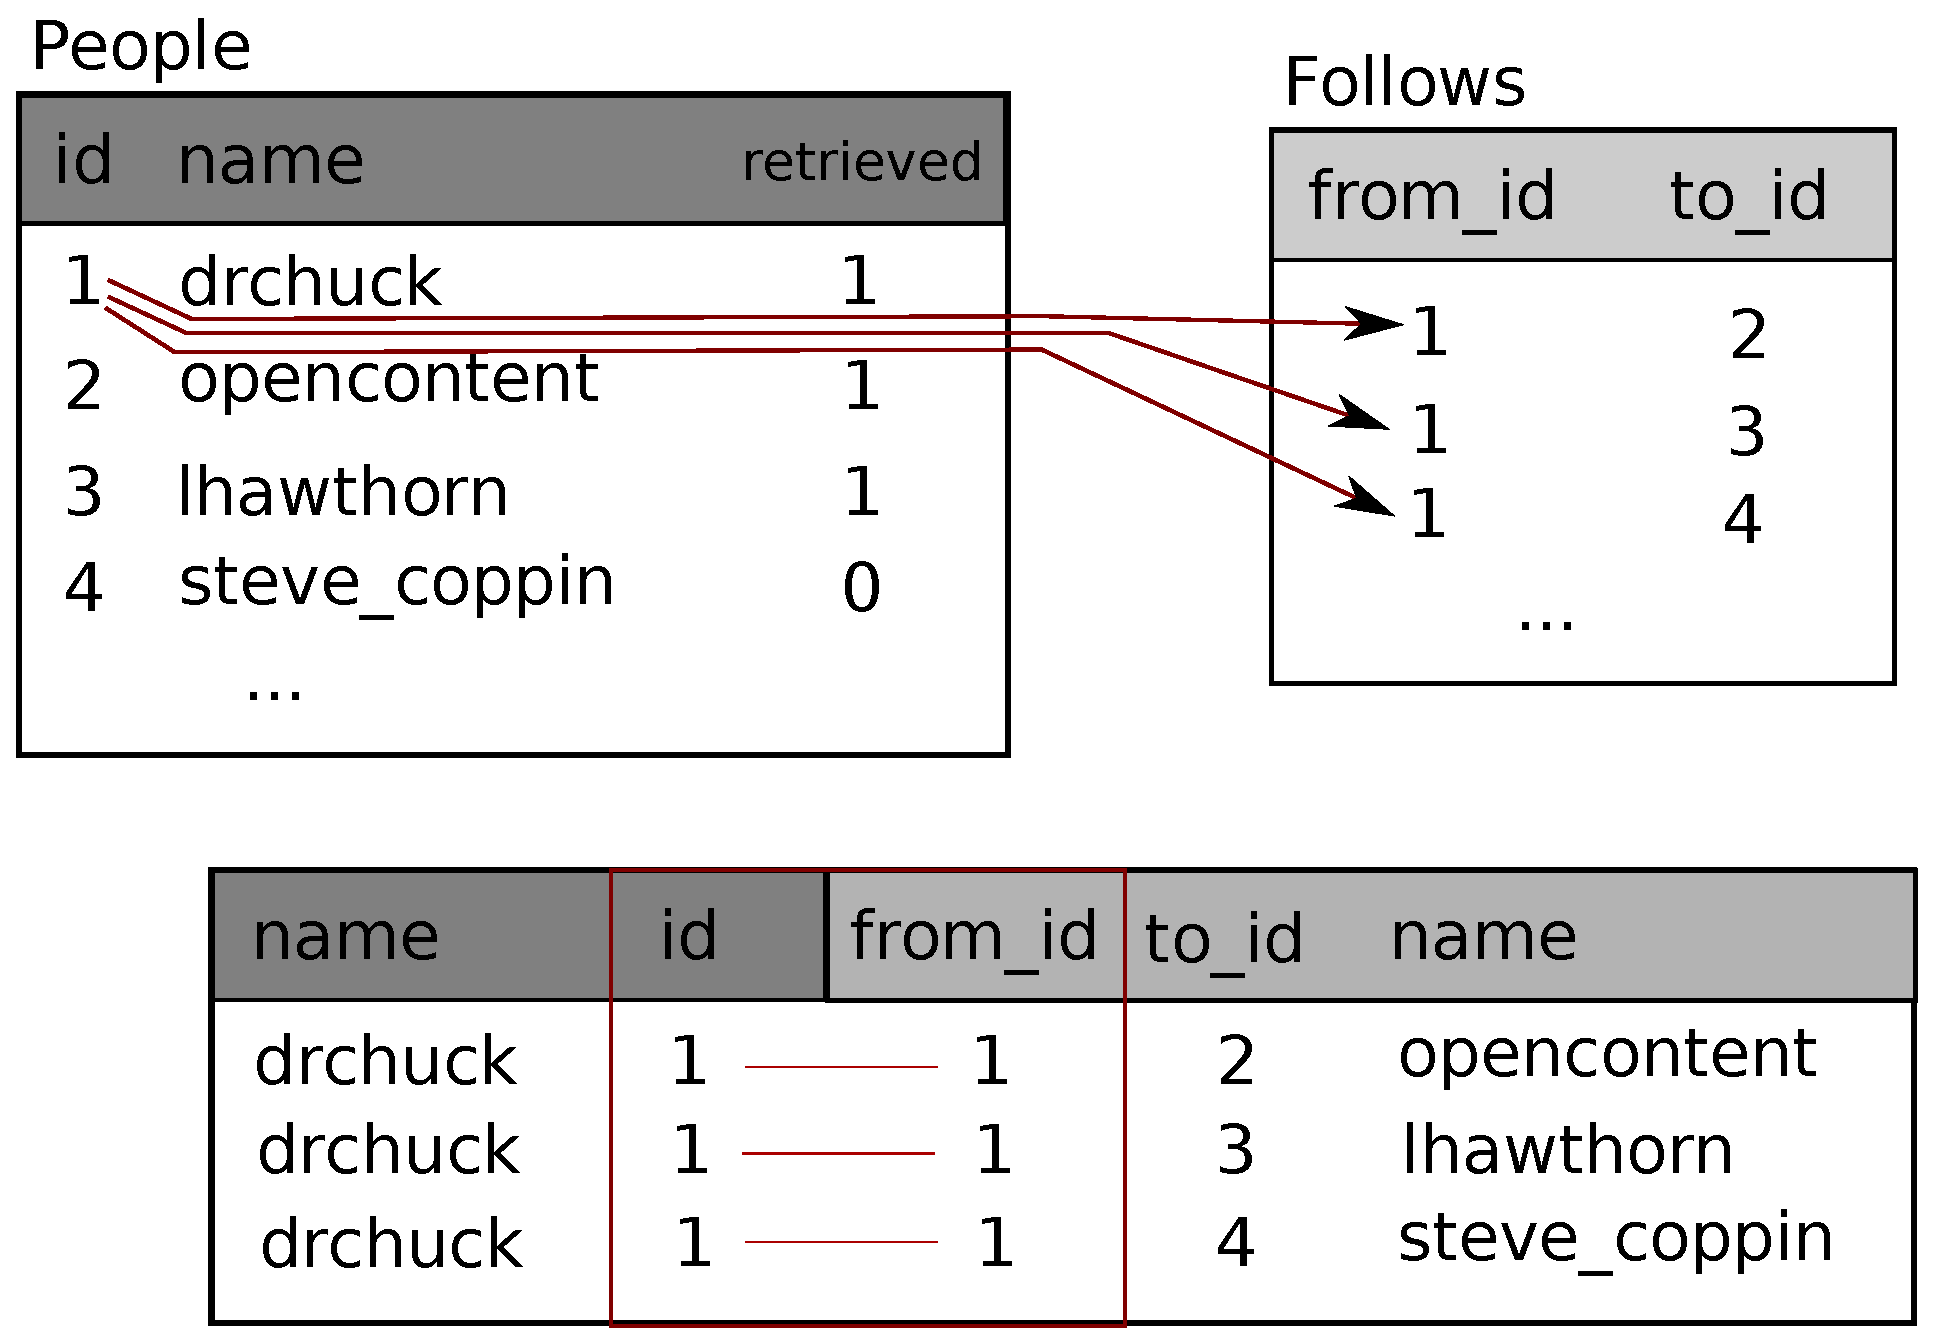
\includegraphics[height=2.50in]{figs2/join.eps}}
\afterfig

The result of the JOIN is to create extra-long ``metarows'' which have both 
the fields from {\tt People} and the matching fields from {\tt Follows}.
Where there is more than one match between the {\tt id} field from {\tt People}
and the \verb"from_id" from {\tt People}, then JOIN creates a metarow 
for \emph{each} of the matching pairs of rows, duplicating data as needed.

The following code demonstrates the data that we will have in the 
database after the multi-table Twitter spider program (above) has
been run several times.

\beforeverb
\begin{verbatim}
import sqlite3

conn = sqlite3.connect('spider.sqlite3')
cur = conn.cursor()

cur.execute('SELECT * FROM People')
count = 0
print 'People:'
for row in cur :
   if count < 5: print row
   count = count + 1
print count, 'rows.'

cur.execute('SELECT * FROM Follows')
count = 0
print 'Follows:'
for row in cur :
   if count < 5: print row
   count = count + 1
print count, 'rows.'

cur.execute('''SELECT * FROM Follows JOIN People 
    ON Follows.to_id = People.id WHERE Follows.from_id = 2''')
count = 0
print 'Connections for id=2:'
for row in cur :
   if count < 5: print row
   count = count + 1
print count, 'rows.'

cur.close()
\end{verbatim}
\afterverb
%
In this program, we first dump out the {\tt People}
and {\tt Follows} and then dump out a subset of the
data in the tables joined together.

Here is the output of the program:

\beforeverb
\begin{verbatim}
python twjoin.py 
People:
(1, u'drchuck', 1)
(2, u'opencontent', 1)
(3, u'lhawthorn', 1)
(4, u'steve_coppin', 0)
(5, u'davidkocher', 0)
55 rows.
Follows:
(1, 2)
(1, 3)
(1, 4)
(1, 5)
(1, 6)
60 rows.
Connections for id=2:
(2, 1, 1, u'drchuck', 1)
(2, 28, 28, u'cnxorg', 0)
(2, 30, 30, u'kthanos', 0)
(2, 102, 102, u'SomethingGirl', 0)
(2, 103, 103, u'ja_Pac', 0)
20 rows.
\end{verbatim}
\afterverb
%
You see the columns from the {\tt People} and {\tt Follows} tables and the last
set of rows is the result of the {\tt SELECT} with the {\tt JOIN} clause.

In the last select, we are looking for accounts that are friends of 
``opencontent'' (i.e., {\tt People.id=2}).

In each of the ``metarows'' in the last select, the first two columns are
from the {\tt Follows}
table followed by columns three through five from the {\tt People} table.  You can also
see that the second column (\verb"Follows.to_id") matches the third column
({\tt People.id}) in each of the joined-up ``metarows''.

\section{Summary}

This chapter has covered a lot of ground to give you an overview of the basics
of using a database in Python.   It is more complicated to write the code to use 
a database to store data than Python dictionaries or flat files so there is 
little reason to use a database unless your application truly needs the capabilities
of a database.  The situations where a database can be quite useful are: 
(1) when your application needs to make small many random updates within a large data set,
(2) when your data is so large it cannot fit in a dictionary and you need to 
look up information repeatedly, or (3) when you have a long-running process that you
want to be able to stop and restart and retain the data from one run to the next.

You can build a simple database with a single table to suit many application 
needs, but most problems will require several tables and links/relationships
between rows in different tables.   When you start making links between 
tables, it is important to do some thoughtful design and follow the 
rules of database normalization to make the best use of the database's
capabilities.  Since the primary motivation for using a database
is that you have a large amount of data to deal with, it is important
to model your data efficiently so your programs run as fast as possible.

\section{Debugging}

One common pattern when you are developing a Python program to connect to
an SQLite database will be to run a Python program and check the
results using the SQLite Database Browser.  The browser allows you 
to quickly check to see if your program is working properly.

You must be careful because SQLite takes care to keep two programs
from changing the same data at the same time.   For example, if
you open a database in the browser and make a change to the database
and have not yet pressed the ``save'' button in the browser, the 
browser ``locks'' the database file and keeps any other program
from accessing the file.  In particular, your Python program
will not be able to access the file if it is locked.

So a solution is to make sure to either close the database browser 
or use the {\bf File} menu to close the database in the browser
before you attempt to access the database from Python to avoid
the problem of your Python code failing because the database is
locked.

\section{Glossary}

\begin{description}

\item[attribute:] One of the values within a tuple.  More commonly
called a ``column'' or ``field''.
\index{attribute}

\item[constraint:] 
When we tell the database to enforce a rule on a field or a row
in a table.  A common constraint is to insist that there can be no
duplicate values in a particular field (i.e., all the values must be unique).
\index{constraint}

\item[cursor:] A cursor allows you to execute SQL commands in a database
and retrieve data from the database.  A cursor is similar to 
a socket or file handle for network connections and files, respectively.
\index{cursor}

\item[database browser:] 
A piece of software that allows you to directly connect to a database 
and manipulate the database directly without writing a program.
\index{database browser}

\item[foreign key:] A numeric key that points to the primary key of 
a row in another table.  Foreign keys establish relationships between rows
stored in different tables.
\index{foreign key}

\item[index:] Additional data that the database software maintains as rows
and inserts into a table to make lookups very fast.
\index{index}

\item[logical key:] A key that the ``outside world'' uses to look up a particular
row.  For example in a table of user accounts, a person's email address
might be a good candidate as the logical key for the user's data. 
\index{logical key}

\item[normalization:] Designing a data model so that no data
is replicated.  We store each item of data at one place in the database
and reference it elsewhere using a foreign key.
\index{normalization}
\index{database normalization}

\item[primary key:] A numeric key assigned to each row that is used to 
refer to one row in a table from another table.  Often the database
is configured to automatically assign primary keys as rows are inserted.
\index{primary key}

\item[relation:] An area within a database that contains tuples and 
attributes.  More typically called a ``table''.
\index{relation}

\item[tuple:] A single entry in a database table that is a set 
of attributes.  More typically called ``row''.
\index{tuple}

\end{description}

